
复杂度是我们衡量一个算法好坏的重要的标准。在算法竞赛中,我们通常关注于算法的时间复杂和空间复杂度。 

一般的来说,复杂度是一个关于输入长度的一个函数。对于某些算法来说,相同的输入的不同输入依然会造成算法的运行时间 / 空间的不同,因此我们通常使用算法的最坏时间复杂度,记为 $T(n)$ 。对于一些特殊的情况,我们可能会关心它的平均情况复杂复杂度(特别是对于随机算法 (randomized algorithm) ),这个时候我们通过使用随机分析 (probabilistic analysis) 来得到期望的复杂度。

\subsection{渐进符号}

我们通常使用渐进符号来描述一个算法的复杂度。

\subsubsection{$\Theta$ 符号}

对于给定的一个函数 $g(n)$, 函数集合 $\Theta(g(n))$ 定义为

$$
\Theta(g(n)) = \{f(n) : 存在常数 c_1,c_2,n_0 \in \mathbb{R^{+}}使得 0 \leq c_1g(n) \leq f(n) \leq c_2g(n), \qquad \forall n \geq n_0\}
$$

也就是说,如果函数 $f(n)$ 属于 $\Theta(g(n))$,那么我们能找到两个正常数 $c_1, c_2$ 使得 $f(n)$ 被 $c_1g(n)$ 和 $c_2g(n)$ 夹在中间。 因为 $\Theta(g(n))$ 是一个函数集合,我们可以用 $f(n) \in \Theta(g(n))$ 表达 $f(n)$ 属于 $\Theta(g(n))$, 但是我们通常使用 $f(n) = \Theta(g(n))$。

\subsubsection{$O$ 符号}

$\Theta$ 符号同时给了我们一个函数的上下界,如果我们只有一个函数的渐进上界的时候,我们使用$O$ 符号。 对于一个给定的函数 $g(n)$, 我们把它记作 $O(g(n))$。

$$
O(g(n)) = \{f(n):存在常数 c,n_0 使得 0\leq f(n) \leq cg(n), \qquad \forall n \geq n_0\}
$$

\subsubsection{$\Omega$ 符号}

同样的,我们使用$\Omega$符号来描述一个函数的渐进下界。

$$
\Omega(g(n)) = \{f(n):存在常数 c,n_0 使得 0 \leq cg(n) \leq f(n) , \qquad \forall n \geq n_0\}
$$

\begin{figure}[h]
\centering
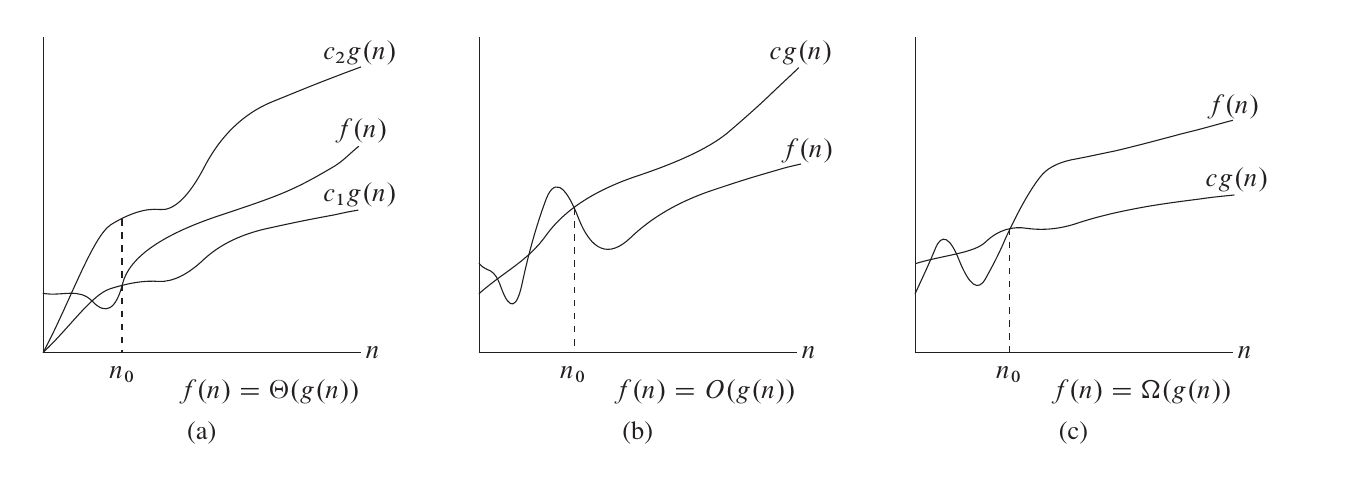
\includegraphics[width=0.5\textwidth]{images/order.png} 

\end{figure}

\subsubsection{常见性质}

\begin{itemize}
\item $f_1(n) + f_2(n) = O(\max(f_1(n), f_2(n)))$
\item $f_1(n) \times f_2(n) = O(f_1(n) \times f_2(n))$
\item 任何对数函数无论底数为何,都具有相同的增长率。$\forall a \neq 1, \log_a{n} = O(\log_2 n)$
\end{itemize}

\subsection{主定理 (Master Theorem)}

我们可以使用 Master Theorem 来快速的求得关于递归算法的复杂度。

假设我们有递推关系式

$$
T(n) = AT\left(\frac{n}{b}\right)+cn^k, \qquad \forall n > b
$$

那么

$$
T(n) = \begin{cases}\Theta(n^{\log_b a}) & a > b^k \\ \Theta(n^k) & a< b^k \\ \Theta(n^k\log n ) & a = b^k \end{cases}
$$

\subsection{均摊复杂度}

算法往往是会对内存中的数据进行修改的,而同一个算法的多次执行,就会通过对数据的修改而互相影响。

例如快速排序中的 “按大小分类” 操作,单次执行的最坏时间复杂度,看似是$O(n)$的。

但是由于快排的分治过程,先前的 “分类” 操作每次都减小了数组长度,所以实际的总复杂度$O(n \log_2 n)$,分摊在每一次 “分类” 操作上,是$O(\log_2 n)$。

多次操作的总复杂度除以操作次数,就是这种操作的\textbf{均摊复杂度}。

\subsection{势能分析}

势能分析,是一种求均摊复杂度下界的方法。

求均摊复杂度,关键是表达出先前操作对当前操作的影响。势能分析用一个函数来表达此种影响。

定义 “状态”$S$:即某一时刻的所有数据。

{\em 在快排的例子中,一个 “状态” 就是当前过程需要排序的下标区间 }

定义 “初始状态”$S_0$:即未进行任何操作时的状态。

{\em 在快排的例子中,“初始状态” 就是整个数组 }

假设存在从状态到数的函数$F$,且对于任何状态$S$,$F(S) \geq F(S_0)$,则有以下推论:

设$S_1,S_2, \cdots ,S_m$为从$S_0$开始连续做$m$次操作所得的状态序列,$c_i$为第$i$次操作的时间开销。

记$p_i = c_i + F(S_i) - F(S_{i-1})$,则$m$次操作的总时间花销为

$$
\sum_{i=1}^m p_i + F(S_0) - F(S_m)
$$

(正负相消,证明显然)

又因为$F(S) \geq F(S_0)$,所以有

$$
\sum_{i=1}^m p_i \geq \sum_{i=1}^m c_i
$$

因此,若$p_i = O(T(n))$,则$O(T(n))$是均摊复杂度的一个下界。

势能分析使用中有很多技巧,案例在此不题。
